\chapter{Случайные блуждания}
\label{ch:chap3}

\textbf{Что такое случайные блуждания?}

Случайное блуждание - последовательность, построенная по следующей рекурентной формуле:

\begin{figure}[H]
    \centering
    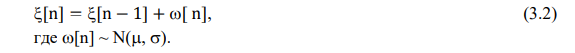
\includegraphics[width=1.0\textwidth]{rand_walk.png}
    \caption{Рекурентная формула случайного блуждания}
\end{figure}

где $\omega[n] = N(u, \sigma)$, а $\xi[0]$ как правило берется равным нулю.\\


\textbf{Чему будет равно математическое ожидание случайного блуждания?}

Если $\xi[0] = 0$, то

$$\xi[n] = \omega_1 + \omega_2 + \omega_3 + ... + \omega_n = N(u, \sigma) + N(u, \sigma) + N(u, \sigma)... = nN(u, \sigma)$$

Логично, что $M\{N(u, \sigma)\} = u$, поэтому

$$M\{\xi[n]\} = nu$$

Если $u$ не равно 0 (как в моем случае), то мат.ожидание линейно зависит от кол-ва измерений (отсчетов). Это лучше всего иллюстрируют
два рисунка ниже:

\begin{figure}[H]
    \centering
    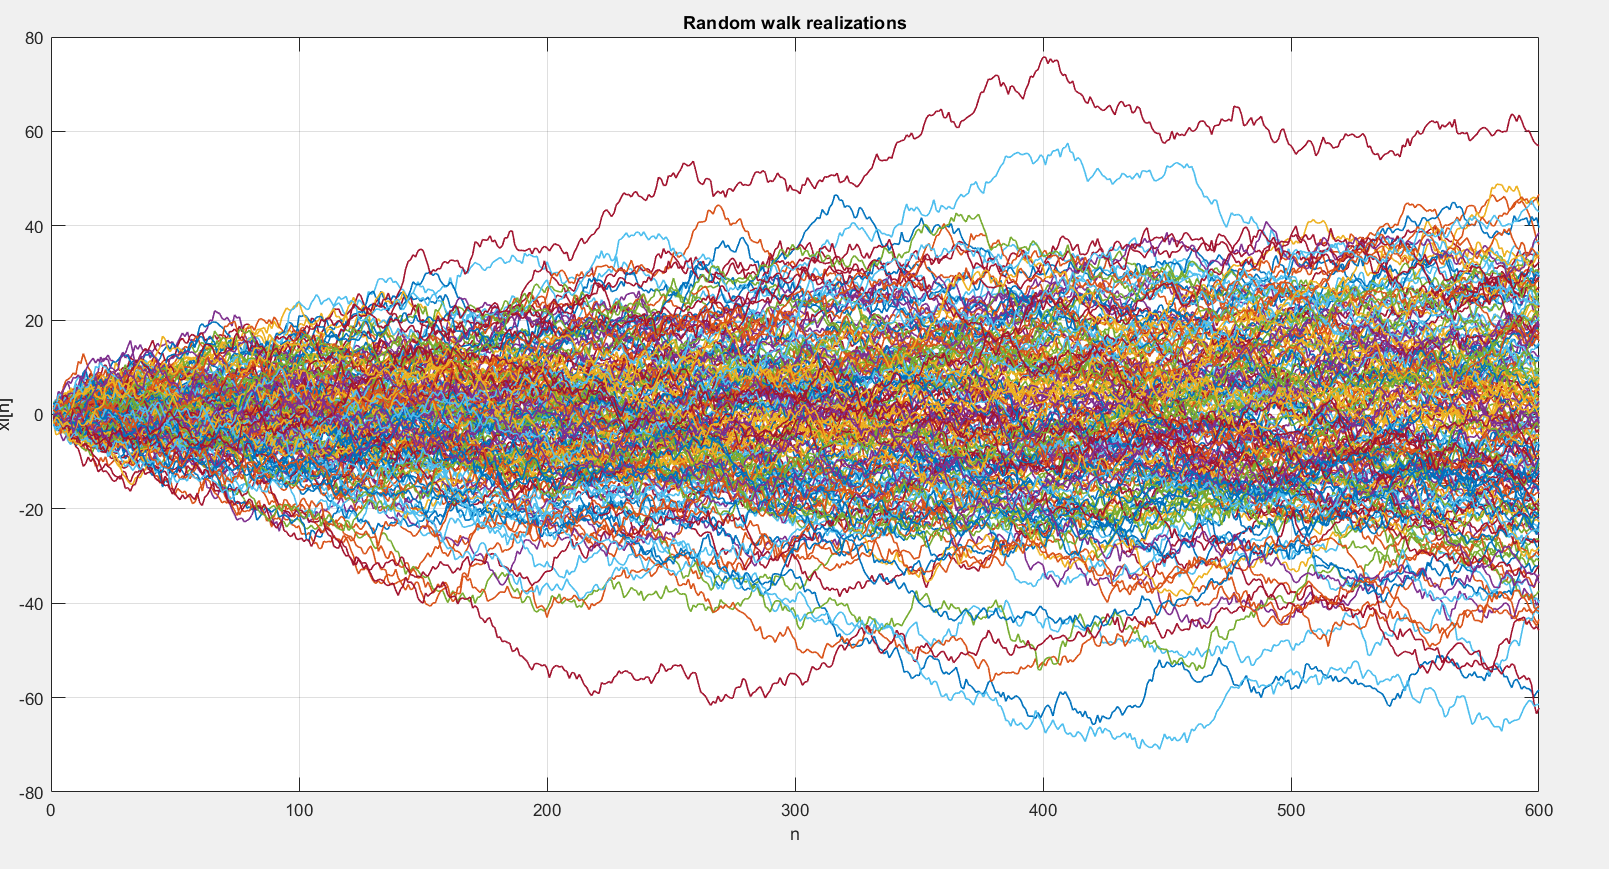
\includegraphics[width=1.0\textwidth]{rwu0.png}
    \caption{Мн-во реализаций СБ при $u$ = 0}
\end{figure}

\begin{figure}[H]
    \centering
    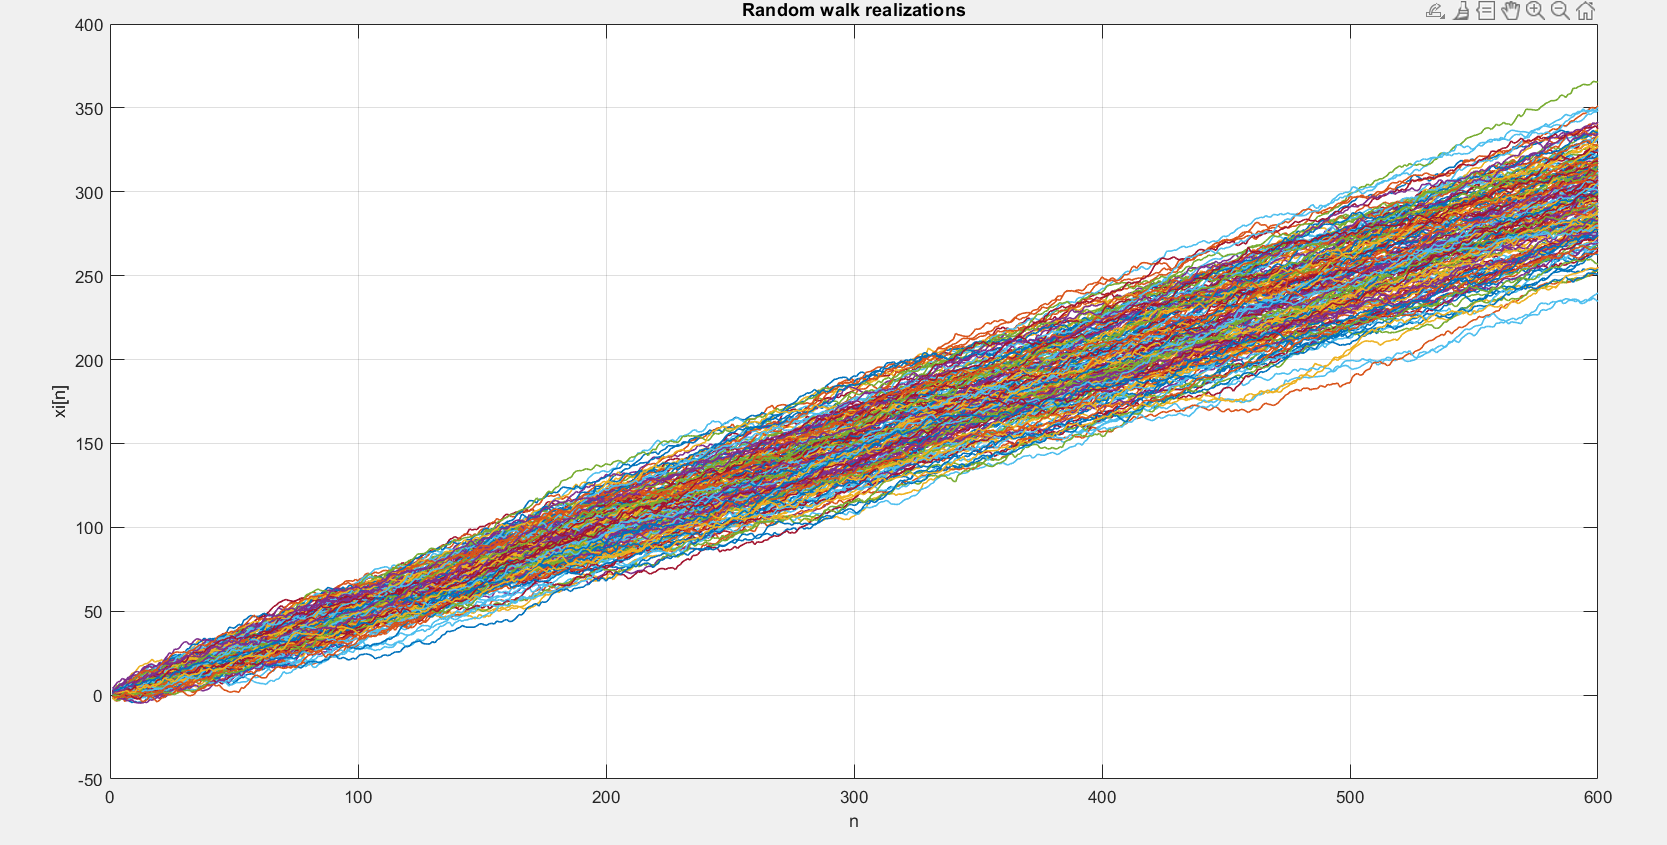
\includegraphics[width=1.0\textwidth]{rwu0.5.png}
    \caption{Мн-во реализаций СБ при $u$ = 0.5}
\end{figure}

Если u не равно 0, то оно будет вести себя, как линейная функция с некоторым наклоном, и значения СБ будет сконцентрированы вокруг
этой наклонной линии.

\textbf{Чему будет равно СКО случайного блуждания?}

Если $\xi[0] = 0$, то

$$\xi[n] = \omega_1 + \omega_2 + \omega_3 + ... + \omega_n = N(u, \sigma) + N(u, \sigma) + N(u, \sigma)... = nN(u, \sigma)$$

$$VAR\{\xi[n]\} = nVAR\{N(u, \sigma)\} = n\sigma^2$$

$$\sigma = \sqrt{n\sigma^2} = \sqrt{n}\sigma$$

Т.к в мое случае $\sigma = 1$, то:

$$\sigma = \sqrt{n}$$

Это значит, что СКО зависит от кол-ва измерений, т.е с увеличением измерений случайное блуждание будет расходиться. В моей программе
кол-во измерений составляет 600. Я увеличу кол-во измерений до 1200 и зафиксирую изменения

\begin{figure}[H]
    \centering
    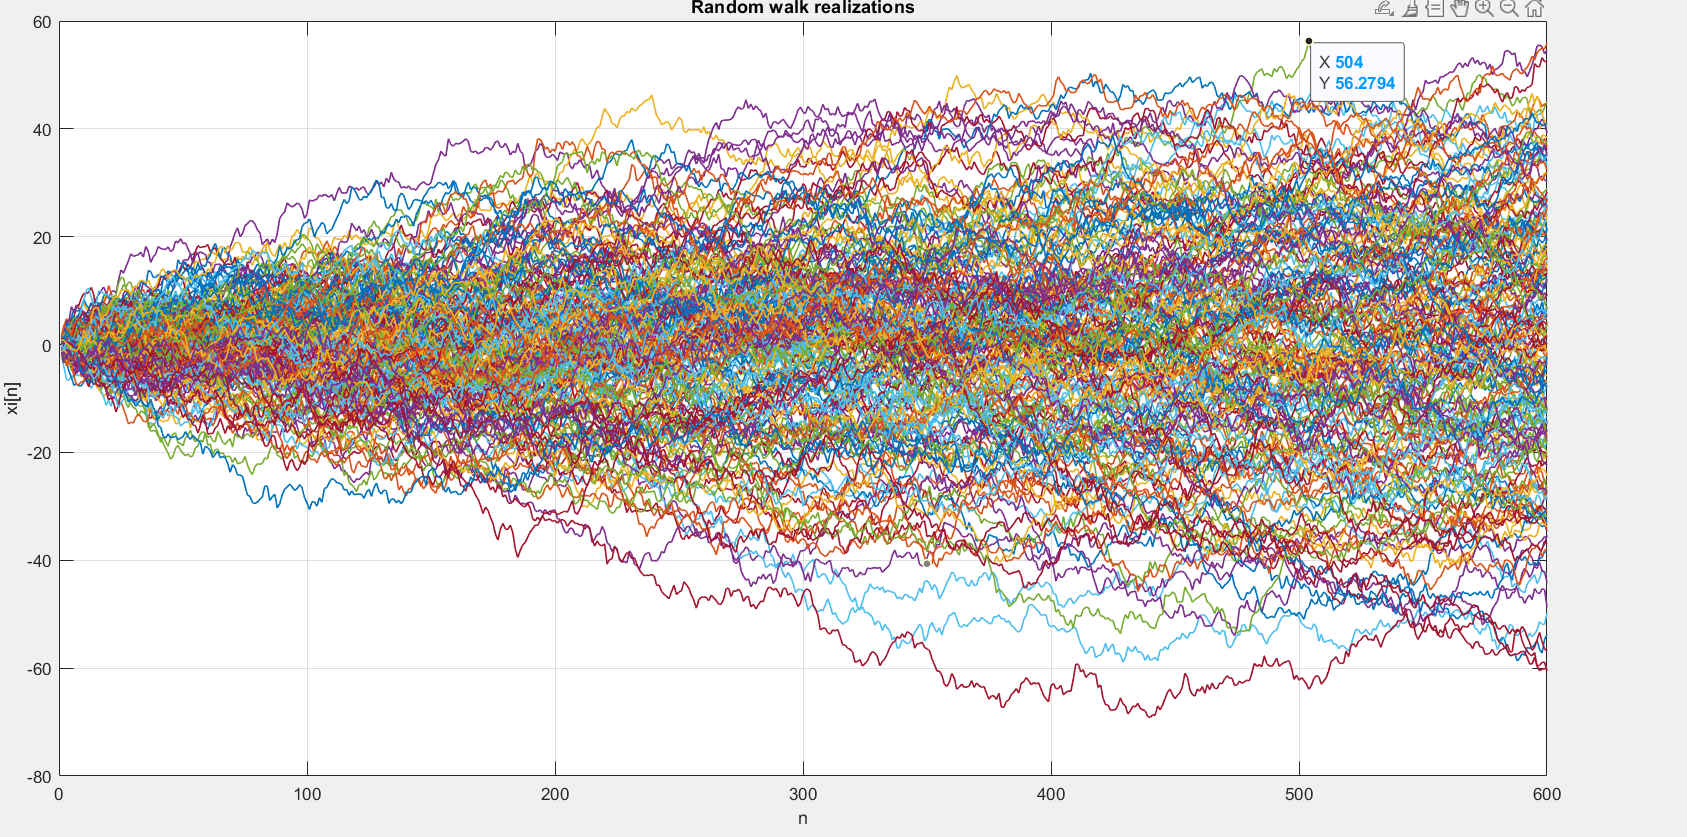
\includegraphics[width=1.0\textwidth]{rwn600.png}
    \caption{Мн-во реализаций СБ при N = 600}
\end{figure}

\begin{figure}[H]
    \centering
    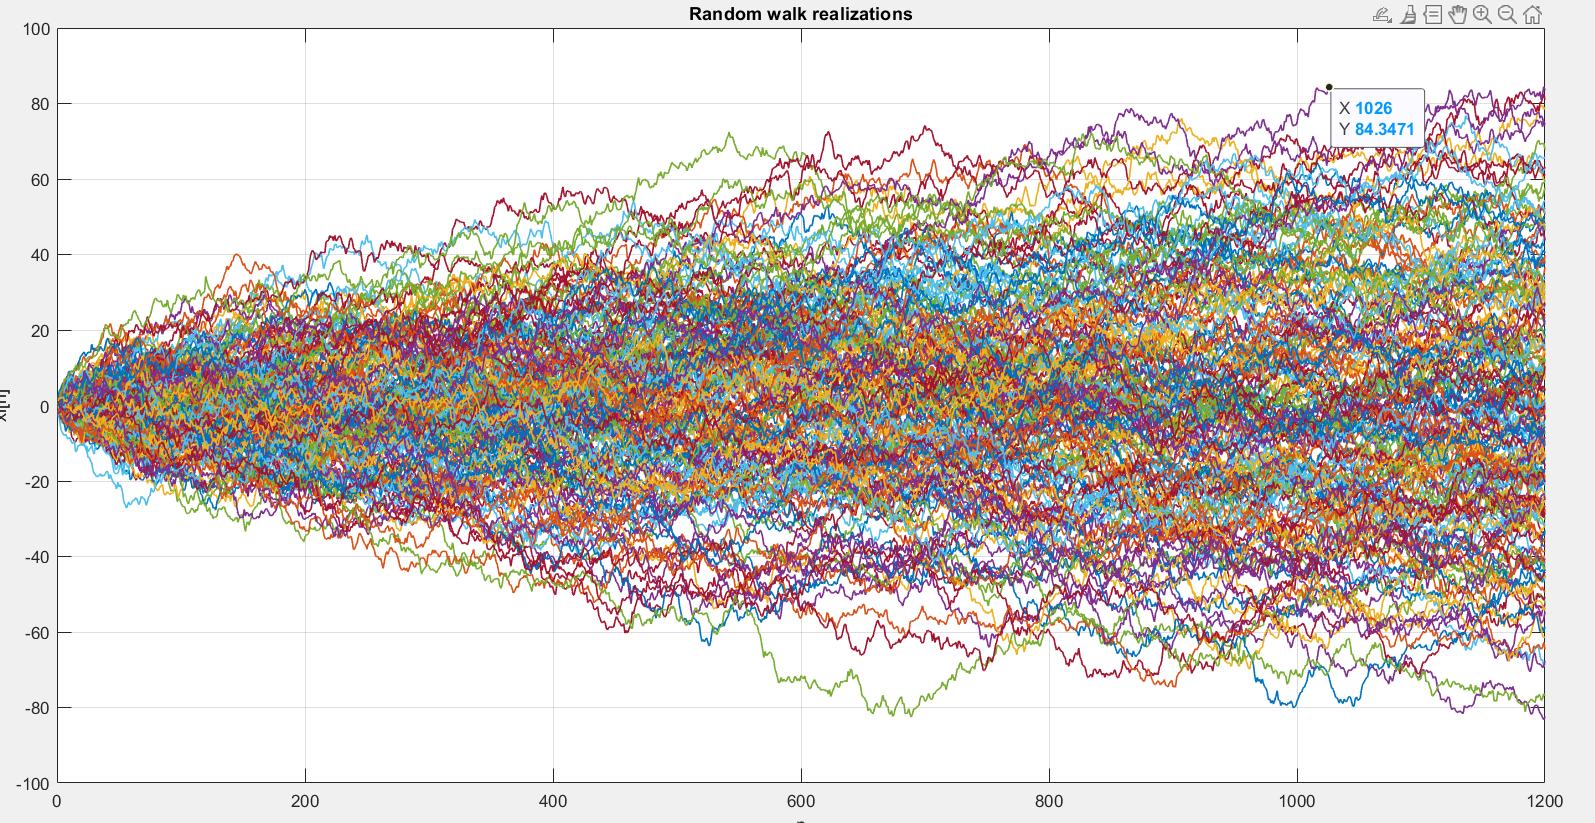
\includegraphics[width=1.0\textwidth]{rwn1200.png}
    \caption{Мн-во реализаций СБ при N = 1200}
\end{figure}

Во втором случае разброс значений (ско) выше, чем в первом, что подтверждает теорию.

\textbf{Чему будет равна автокорреляция случайного блуждания?}

Автокорреляция - корреляция между соседними точками процесса. \\

В нашем случае автокорреляция будет следующая:

$$r = M\{\xi[n]*\xi[n-1]\}$$

Заметим, что $\xi[n] = \xi[n-1] + \omega_1$, тогда

$$r = M\{(\xi[n-1] + \omega_1)*\xi[n-1]\} = M\{(\xi[n-1])^2\} + M\{\xi[n-1]\omega_1\}$$

Заметим, что $M\{(\xi[n-1])^2\} = VAR\{\xi[n-1]\} = (n-1)\sigma^2, M\{\omega_1\} = u, M\{\xi[n-1]\} = (n-1)u$, тогда

$$r = (n-1)\sigma^2 + (n-1)u^2 $$

В моем случае  u = 0, поэтому

$$r = (n-1)\sigma^2$$

Из этого можно сделать вывод, что в случайном блуждании автокорреляция зависит от n (момента времени или отсчета), а это значит,
что процесс не стационарен, т.е будет изменять свои параметры с течением времени.

При лаге l > 0 получим такую же формулу:

$$r = (n-l)\sigma^2$$

Если захотим вычислить нормированный коэффициент корреляции, то получим

\[
\rho_{\xi}(n, n-l) = \frac{r_{\xi}(n, n-l)}{\sqrt{\mathrm{Var}[\xi[n]] \, \mathrm{Var}[\xi[n-l]]}}
= \frac{n\sigma_\omega^2}{\sqrt{\,n\sigma_\omega^2 \cdot (n-l)\sigma_\omega^2\,}}
= \sqrt{\frac{n-l}{n}}.
\]

При $n ->\infty$ и фиксированном l выражение сверху будет стремиться к 1. Это значит, что с течением времени все соседние значения
будут полностью зависимы.

Построим скаттерограммы (диаграммы рассеяния) случайного блуждания с лагами l = 1 и l = 10

\begin{figure}[H]
    \centering
    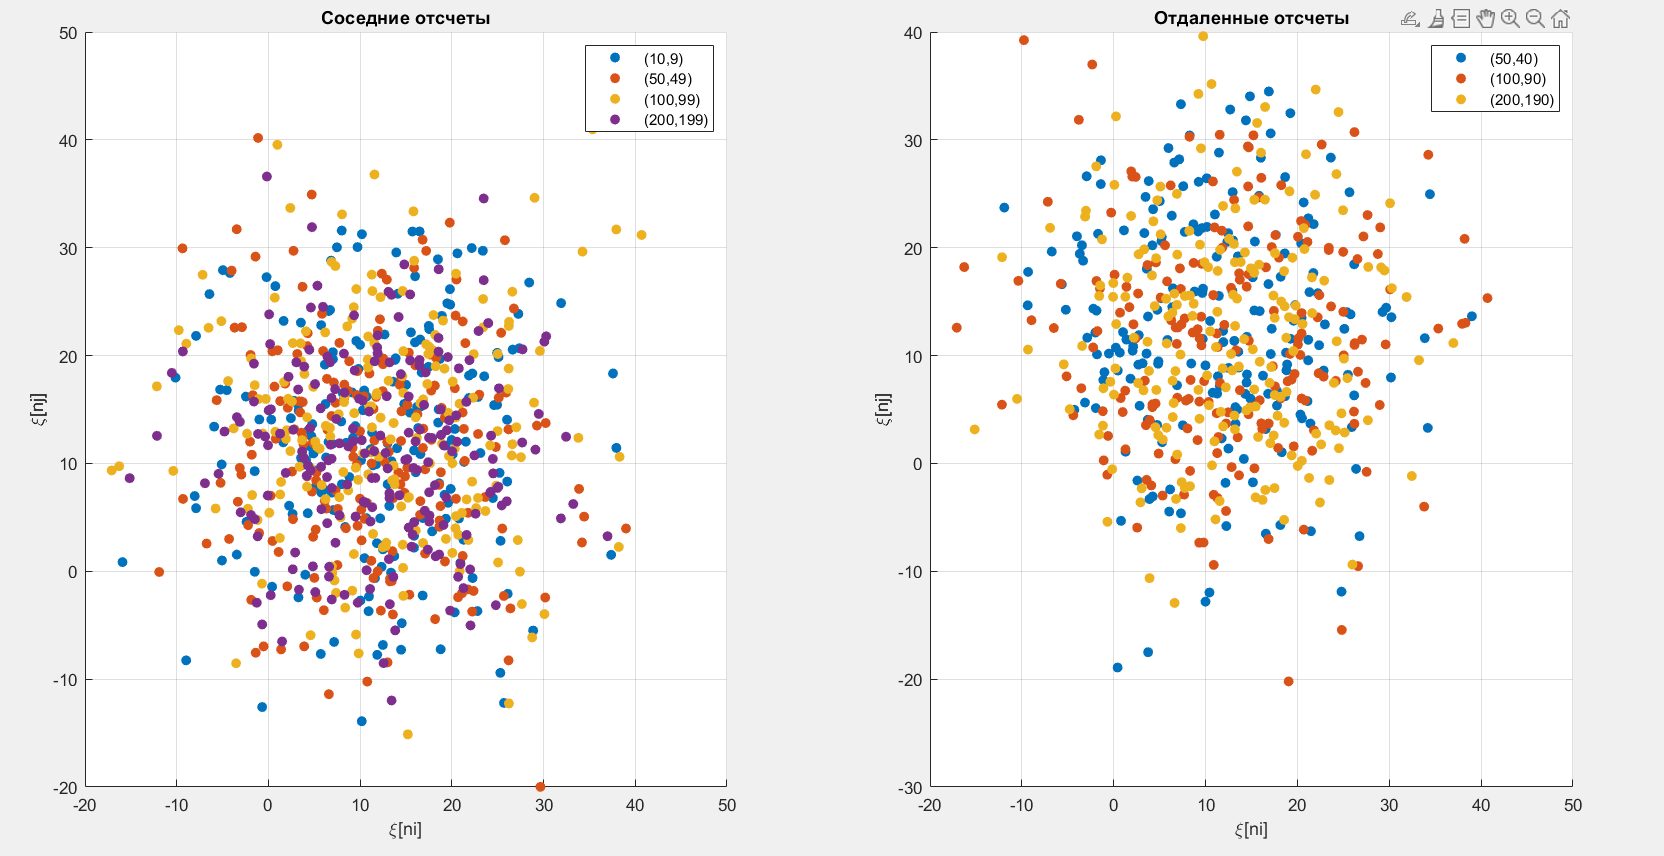
\includegraphics[width=1.0\textwidth]{rwscat.png}
    \caption{Скаттерограммы для СБ с разными лагами}
\end{figure}

На графике слева точки более плотно сгруппированы возле диагонали, что указывает на более высокий коэффициент корреляции относительно
графика справа. Это подтверждает теоретическую формулу о корреляции, т.к с увеличением лага уменьшается корреляция.


\endinput